\documentclass[12pt, letterpaper]{report}
\usepackage[utf8]{inputenc}
\usepackage{graphicx}

\graphicspath{{./images/}}

\begin{document}

%- Requirements
%	Problem Statement
%	Constraints
%	Requirements
%	HW and SW Specification
%	Analysis Verification
\chapter{Introduction}
\section{Problem Statement}
Due to COVID-19 [ref], many countries established mandatory lockdown, which increased the usage of entertainment platforms. Television continues to have an important role in this matter, and that’s why a better user experience, through a good interface, is increasingly needed.
Despite knowing that smart TV’s market is growing, because of its features, a large percentage of the televisions in use are non-smart TV’s [ref], which use infrared sensors to allow the user to control the TV, via a remote control. In this report, it will be analyzed and designed a remote control with the following characteristics: it must control the TV using an infrared sensor, it must be light and battery powered. It should have three buttons: one to switch the TV on/off, called “Power”; the other two buttons are used to scroll up/down and select the available channels, and they are labeled with the arrows up/down, respectively. The main goal of this project is to consolidate the methods of the Waterfall model, as it is a classic model in software development methodology, suitable for small-scale projects.

\section{Problem Statement Analysis}
In order to have a better and deeper understanding of the problem, it’s essential to identify the entities involved and their relationships. Using that analysis, a system diagram can be built, [ref], relating the known entities and presenting some attributes.

\begin{figure}[ht]
	\centering
	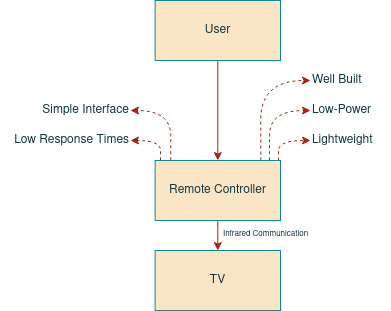
\includegraphics[width=0.75\textwidth]{prob_statement}
	\caption{Problem Statement Analysis Diagram}
	\label{fig:prob_statement}
\end{figure}

This image [ref] shows that the remote controller is the only interface between the user and the TV. The user interacts with the remote by pressing one of the existing buttons, and in turn, the remote interacts with the television via an infrared beam. Knowing that the remote controller must have a long lifespan, it must be well built, in order to resist eventual falls, and also, it must have a low consumption, in order to avoid the frequent change of batteries. For a better user experience, the remote should be lightweight, have a simple interface and respond quickly to user commands.

\chapter{Analysis}
\section{Market Research}
\subsection{Market Definition}
A remote control, by definition, is an electronic device used to operate another device from a distance, usually wirelessly. These allow you to control different types of devices, such as televisions, air conditioning, DVD players, sound systems, among others. Remote controllers have different technologies to communicate with the devices they control, such as Bluetooth, Wi-Fi, Radio Frequency (RF) and Infrared (IR), the latter being the most used technology in remote controls.

There are three types of remotes:

\begin{itemize}
	\item Dedicated Remote: a remote programmed to control one or more 					specific devices; 

	\item Universal Remote Control: also called a ‘library’ remote, it’s 				programmed by manufacture to control almost all common home devices;

	\item Programmable Remote Control: can be programmed either with codes 				to control devices or create more elaborate functions via a 					computer or mobile app, using USB communication, Bluetooth or Wifi.
\end{itemize}

Regarding the application field, since this allows the operation of devices that are out of convenient reach for direct operation of controls, they may be used in different fields, like industry, civil, military, space, and others.

\subsection{Bench-Marking}
Most of the time, when you buy a device that requires a remote control, it's already included. In the table below [ref], there are shown some of the most popular remotes in the market right now.

\begin{table}[h]
	\centering
	\begin{tabular}{||c c c c c||} 
	\hline
	Product Name & Price (€) & Weight (g) & Comm. Technology & Remote Type\\
	\hline\hline
	Roku Voice & 17,30 & 90,72 & Wi-Fi & Dedicated\\ 
	Apple TV & 25,00 & 18,14 & Wi-Fi, Bluetooth & Dedicated \\
	DIRECTV RC73 & 6,05 & 90,71 & IR, RF & Programmable\\
	IR-1316 & 12,97 & 49,89 & IR & Universal\\
	\hline
\end{tabular}
				
\caption{Most popular Amazon's remote controllers. }
\label{table:popular_remotes}
\end{table}
		
\section{System}
\subsection{System Overview}
As shown in [fig], the push buttons on the remote behave as sensors, which produce an electrical signal whenever they are pressed. This electrical signal is processed by the controller, transmitting to the infrared emitter (actuator) a signal identifying the operation performed by the user. 

[FIGURE]

\subsection{System Requirements and Constraints}

Functional Requirements:
\begin{itemize}
	\item Three push buttons.
\end{itemize}

Non-Functional Requirements:
\begin{itemize}
	\item Lightweight;
	\item Low-Power consumption;
	\item Well built;
	\item Simple interface;
	\item Low response times.
\end{itemize}

System Constraints:
\begin{itemize}
	\item Time constraint;
	\item 2 Members team;
	\item Infrared communication.
\end{itemize}
\subsection{Hardware and Software Specification}

\section{Analysis Verification}


%- Design
%	Analysis Review
%	HW Components Specification
%	Defining HW interface
%	SW Components Specification
%	Defining SW interface
%	Start-up/shutdown process Specification
%	Errors Handling Specification
%	Design Verification


\end{document}